\section{การออกแบบส่วนติดต่อของผู้ใช้ (User Interface)}

การออกแบบส่วนติดต่อของผู้ใช้ในแอปพลิเคชัน มีดังนี้
\subsection{หน้าเข้าสู่ระบบ}
หน้าเข้าสู่ระบบ จะแสดงขึ้นเมื่อผู้ใช้เข้าสู่แอปพลิเคชัน ผู้ใช้จะต้องกรอก Email และ Password ที่ได้ลงทะเบียนไว้ จากนั้นจึงกด Sign In เพื่อเข้าสู่ระบบ
\begin{figure}
    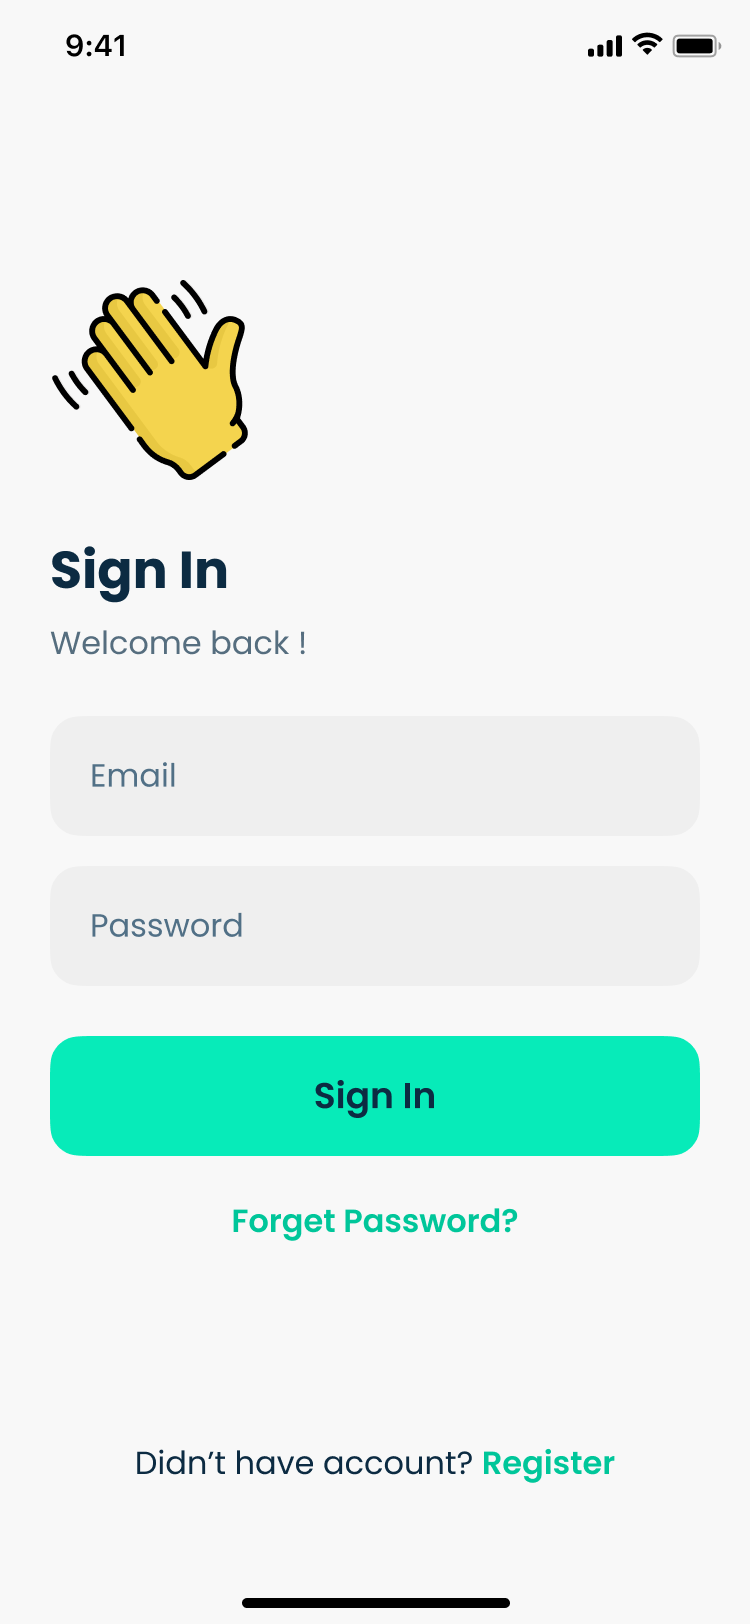
\includegraphics[height=10cm]{chapter_3/ui/Sign In.png}
    \caption{หน้าเข้าสู่ระบบ}
\end{figure}

\subsection{หน้าลงทะเบียน}
หน้าลงทะเบียน จะให้ผู้ใช้กรอกข้อมูลต่าง ๆ ดังนี้
\begin{enumerate}
    \item Email ที่จะใช้ลงทะเบียน
    \item Password ของบัญชี
\end{enumerate}
\begin{figure}
    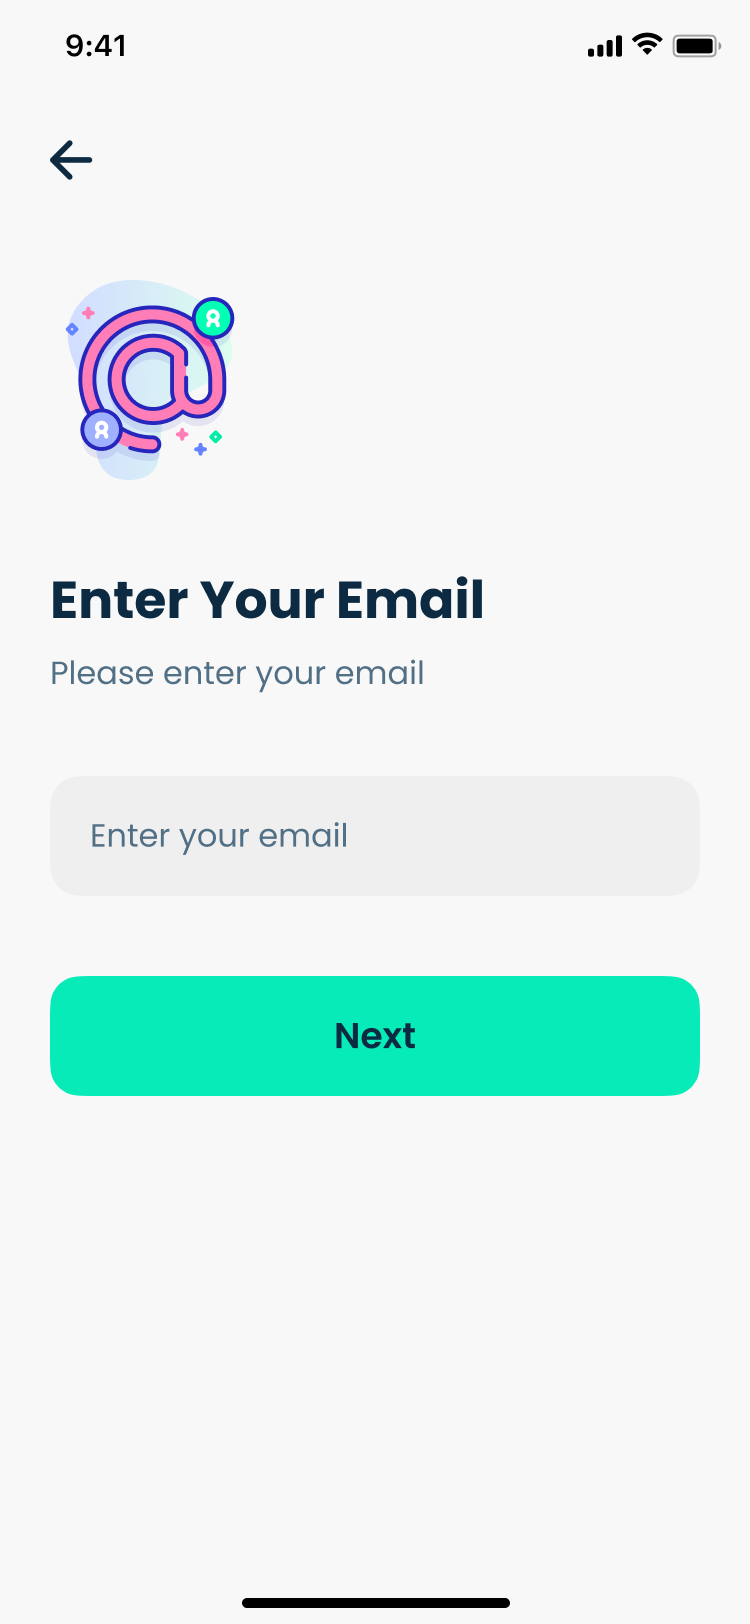
\includegraphics[height=10cm]{chapter_3/ui/Register/Email.png}
    \caption{หน้าการกรอก Email ที่จะใช้ลงทะเบียน}
\end{figure}
\begin{figure}
    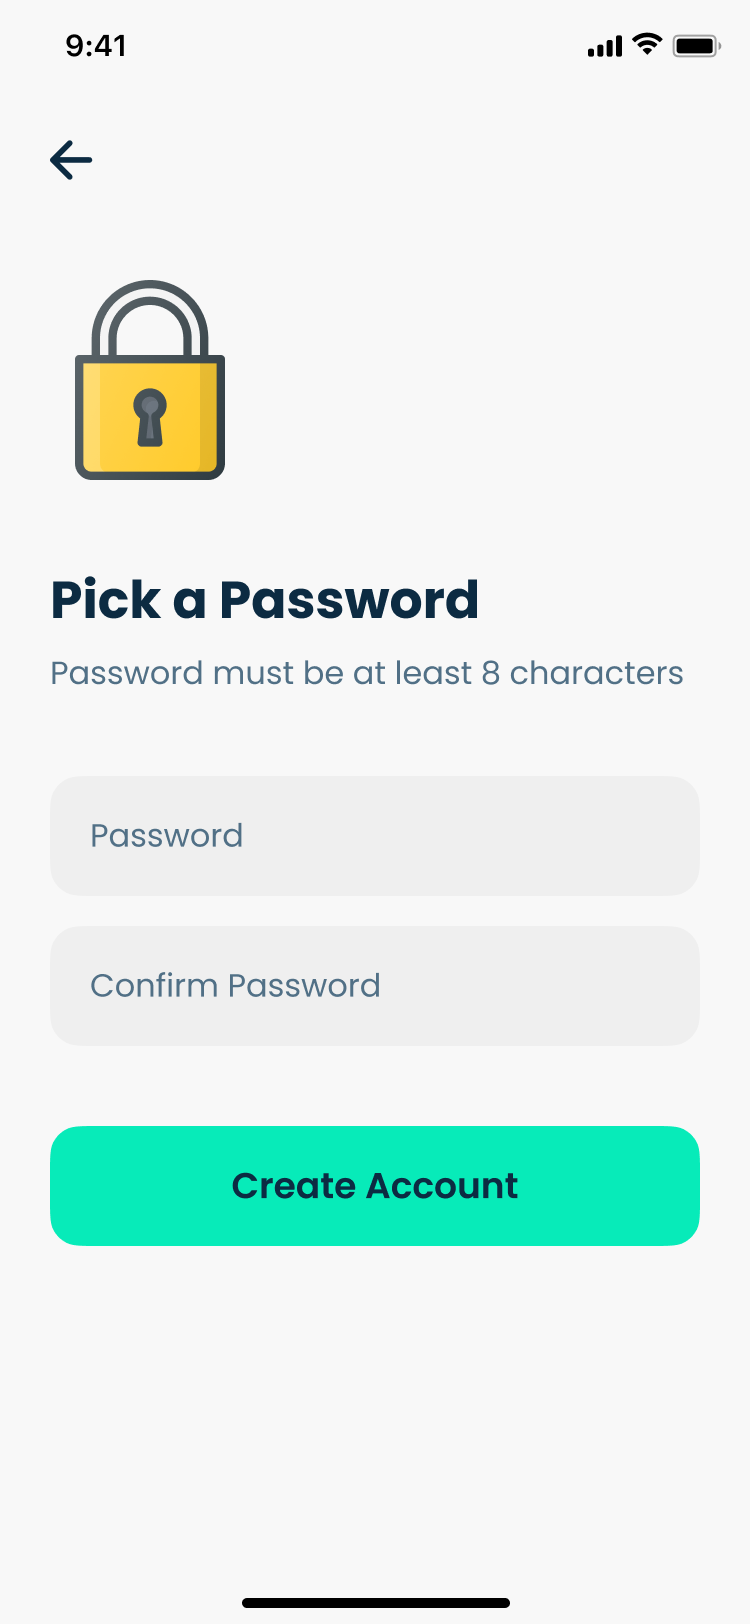
\includegraphics[height=10cm]{chapter_3/ui/Register/Password.png}
    \caption{หน้าการกำหนดรหัสผ่าน}
\end{figure}
\begin{figure}
    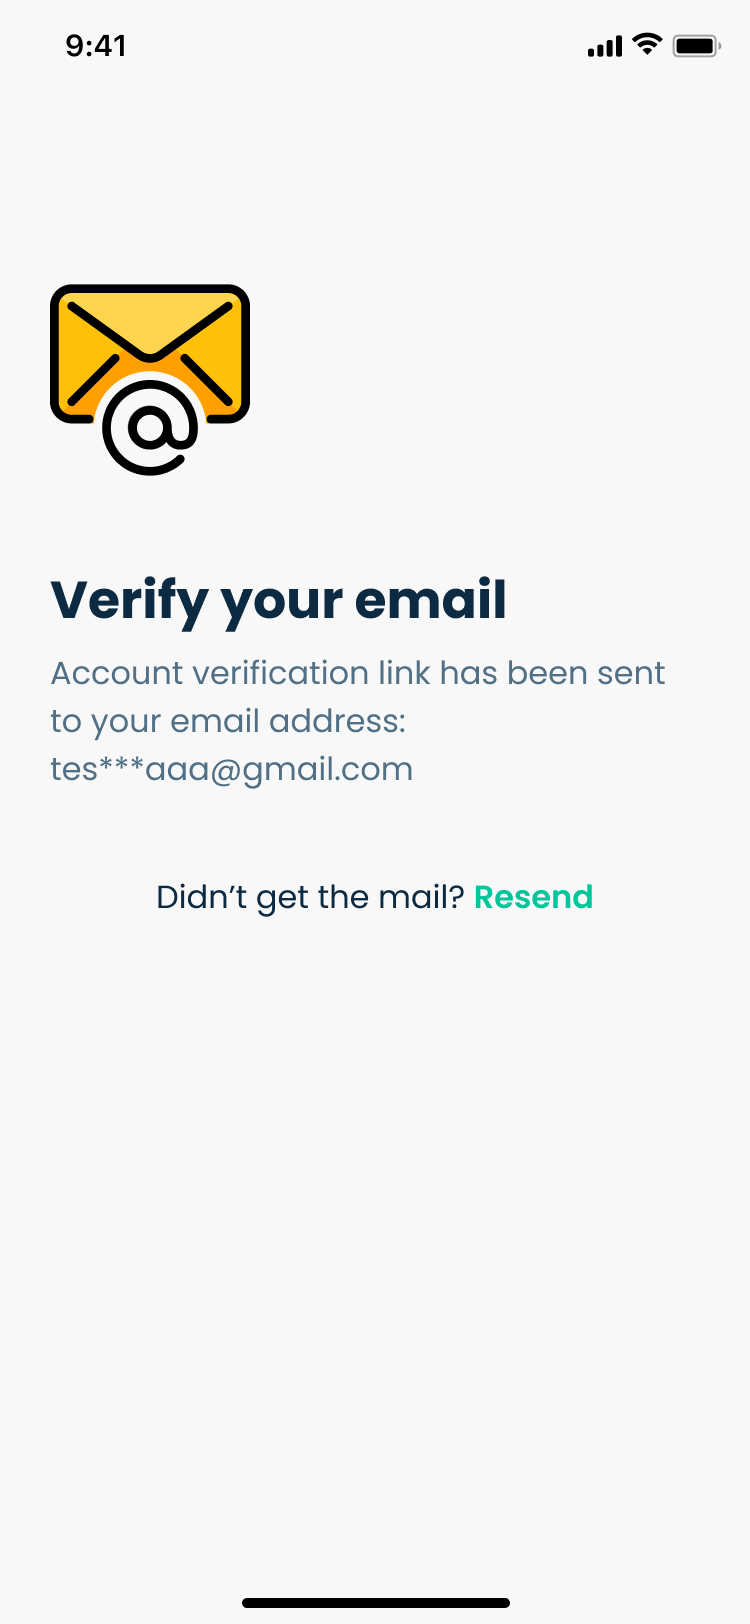
\includegraphics[height=10cm]{chapter_3/ui/Register/Email Verification.png}
    \caption{หน้าการ Verify อีเมล}
\end{figure}
\indent จากนั้น ระบบจะแจ้งให้ผู้ใช้ยืนยัน Email ที่ได้กรอกไว้ ซึ่งจะให้ผู้ใช้ตรวจสอบ Email ที่ระบบได้ส่งไป เมื่อผู้ใช้ยืนยันตัวตนเรียบร้อยแล้ว 
แอปพลิเคชันจะให้ผู้ใช้กรอกข้อมูล ดังนี้
\begin{enumerate}
    \item Display Name สำหรับบัญชีผู้ใช้ ซึ่งจะใช้ในการให้ผู้อื่นสามารถค้นหาบัญชีได้
    \item Profile Picture ให้ผู้ใช้อัปโหลดรูปโปรไฟล์ของตัวเอง ซึ่งผู้ใช้สามารถข้ามขั้นตอนนี้ได้
\end{enumerate}
\begin{figure}
    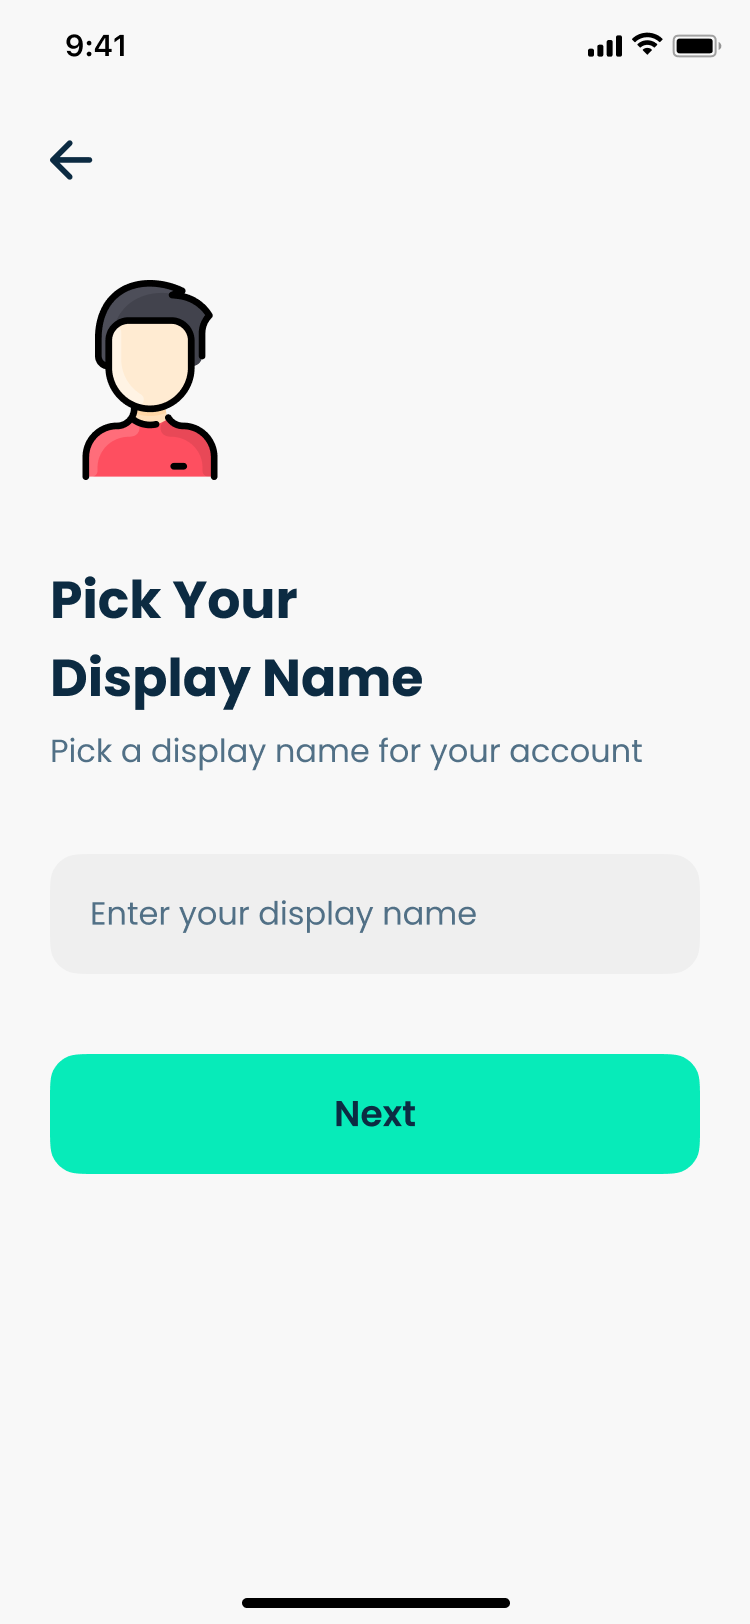
\includegraphics[height=10cm]{chapter_3/ui/Register/Display Name.png}
    \caption{หน้าการกรอก Display Name}
\end{figure}
\begin{figure}
    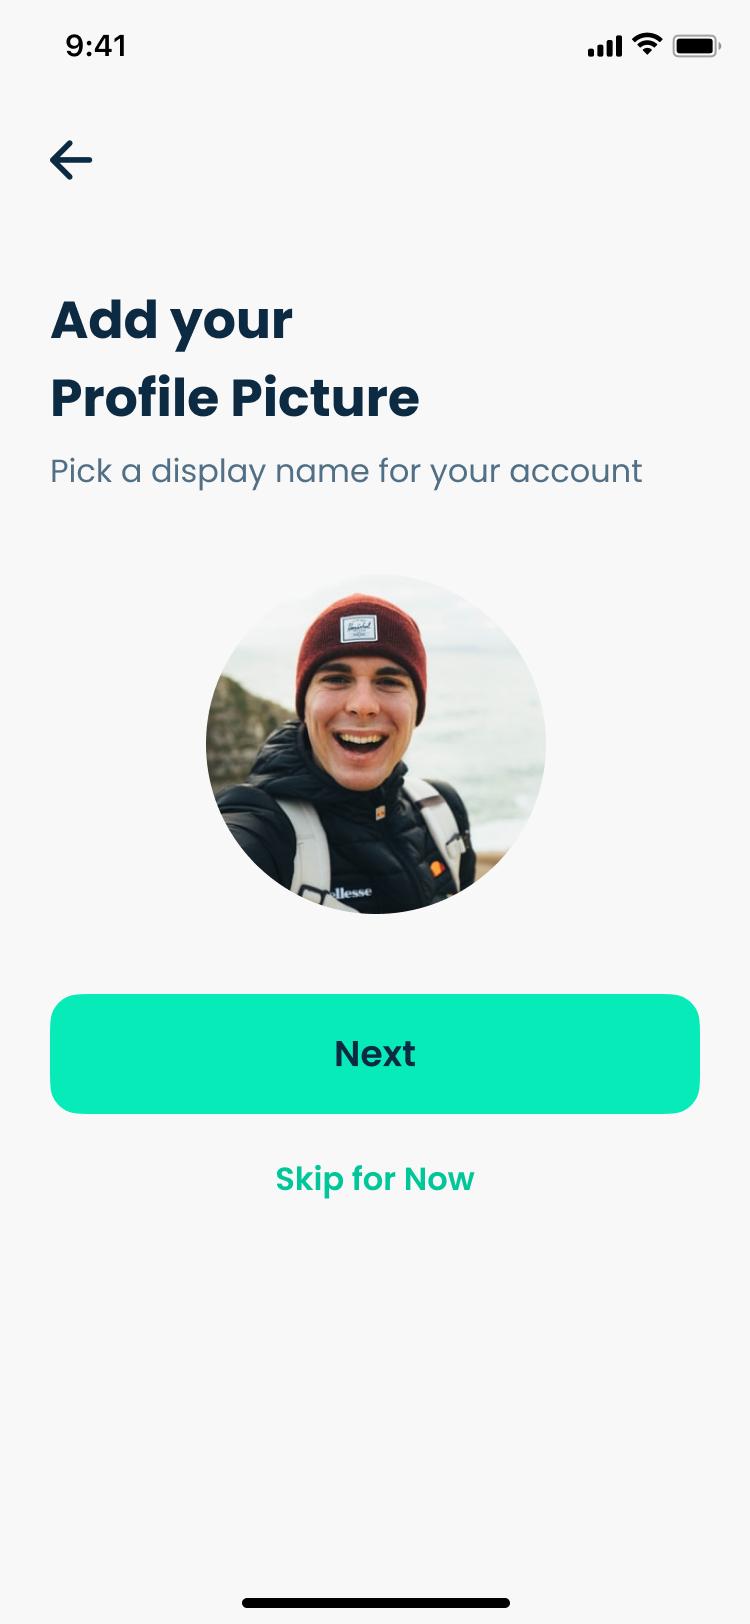
\includegraphics[height=10cm]{chapter_3/ui/Register/Profile Picture.png}
    \caption{หน้าการเพิ่มรูปภาพของผู้ใช้}
\end{figure}

\subsection{หน้าหลังจากการลงทะเบียน}
เมื่อผู้ใช้ลงทะเบียนเรียบร้อยแล้ว ระบบจะถามคำถามต่าง ๆ เพื่อให้ระบบทราบถึงความต้องการในการออกกำลังกาย และสามารถแนะนำคอร์สออกกำลังกายได้แม่นยำมากขึ้น ซึ่งระบบจะถามคำถาม ดังนี้
\begin{enumerate}
    \item เพศของผู้ใช้
    \item ปีเกิดของผู้ใช้
    \item น้ำหนักและส่วนสูงของผู้ใช้
    \item ประเภทของการออกกำลังกายที่ชื่นชอบ
    \item ส่วนของร่างกายที่ต้องการหลีกเลี่ยง
\end{enumerate}

\begin{figure}
    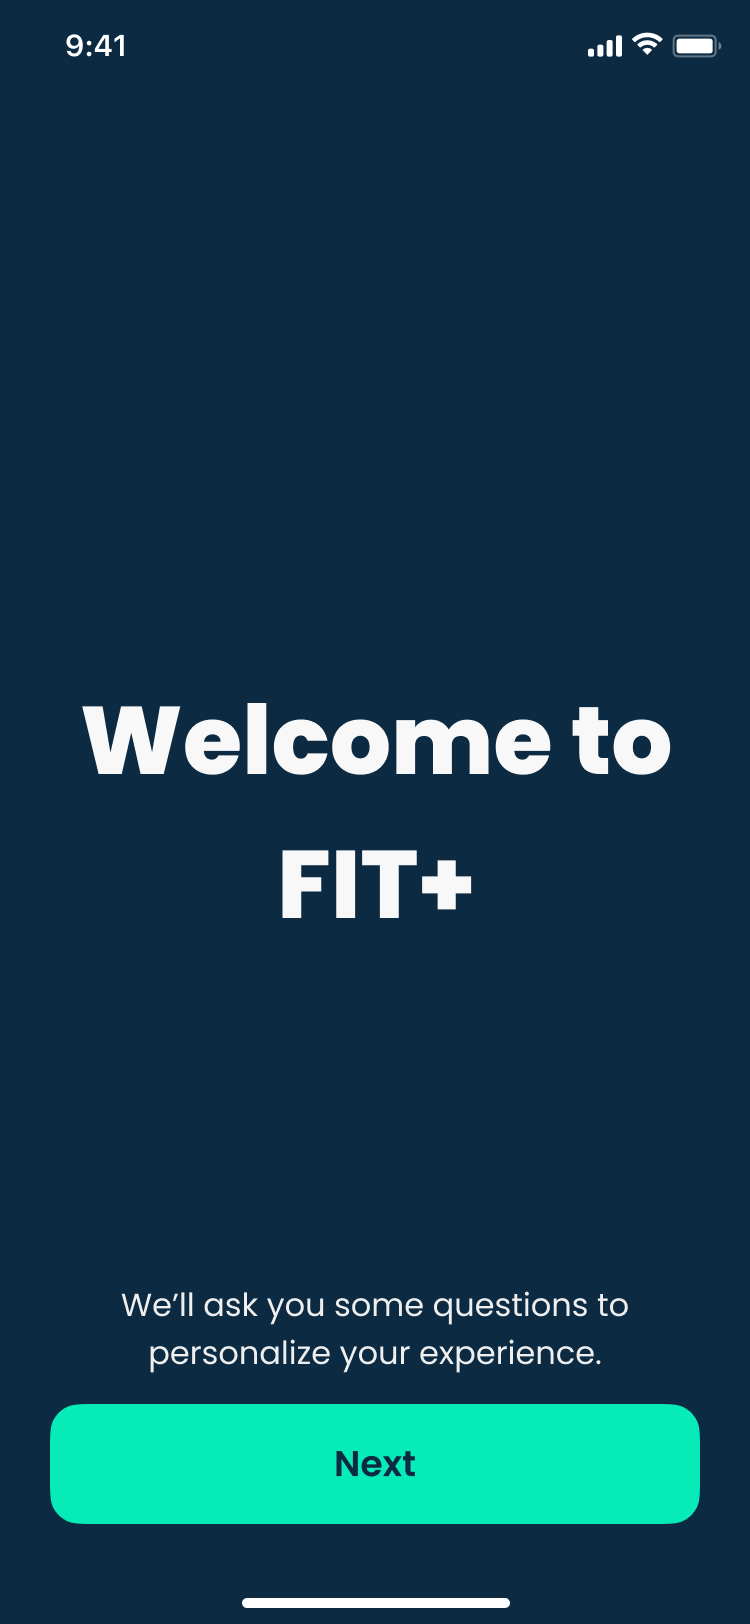
\includegraphics[height=10cm]{chapter_3/ui/New User Setup/000 - Welcome.png}
    \caption{หน้าหลังจากการยืนยันตัวตนเรียบร้อยแล้ว}
\end{figure}
\begin{figure}
    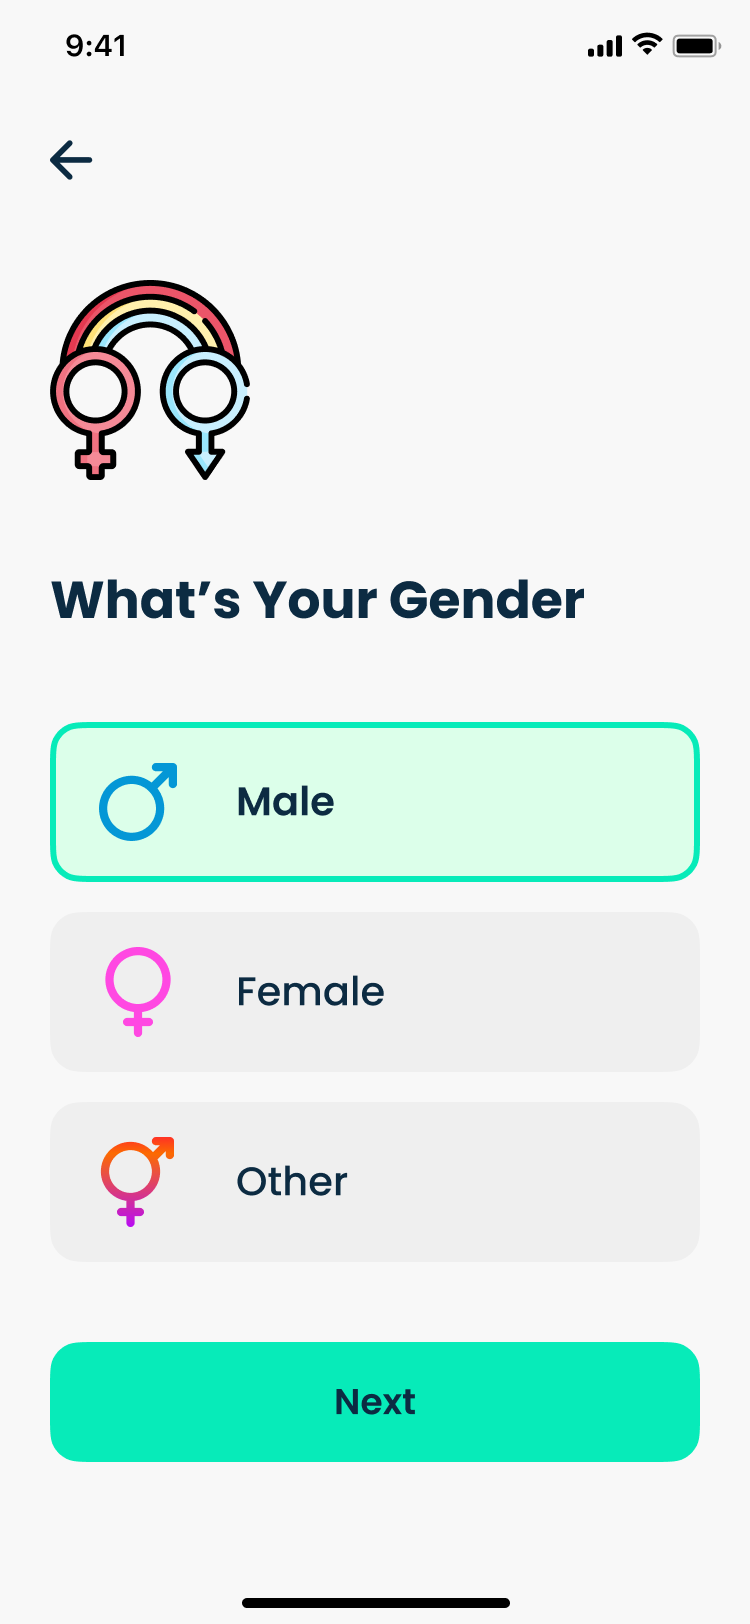
\includegraphics[height=10cm]{chapter_3/ui/New User Setup/001 - Gender.png}
    \caption{หน้าการระบุเพศ}
\end{figure}
\begin{figure}
    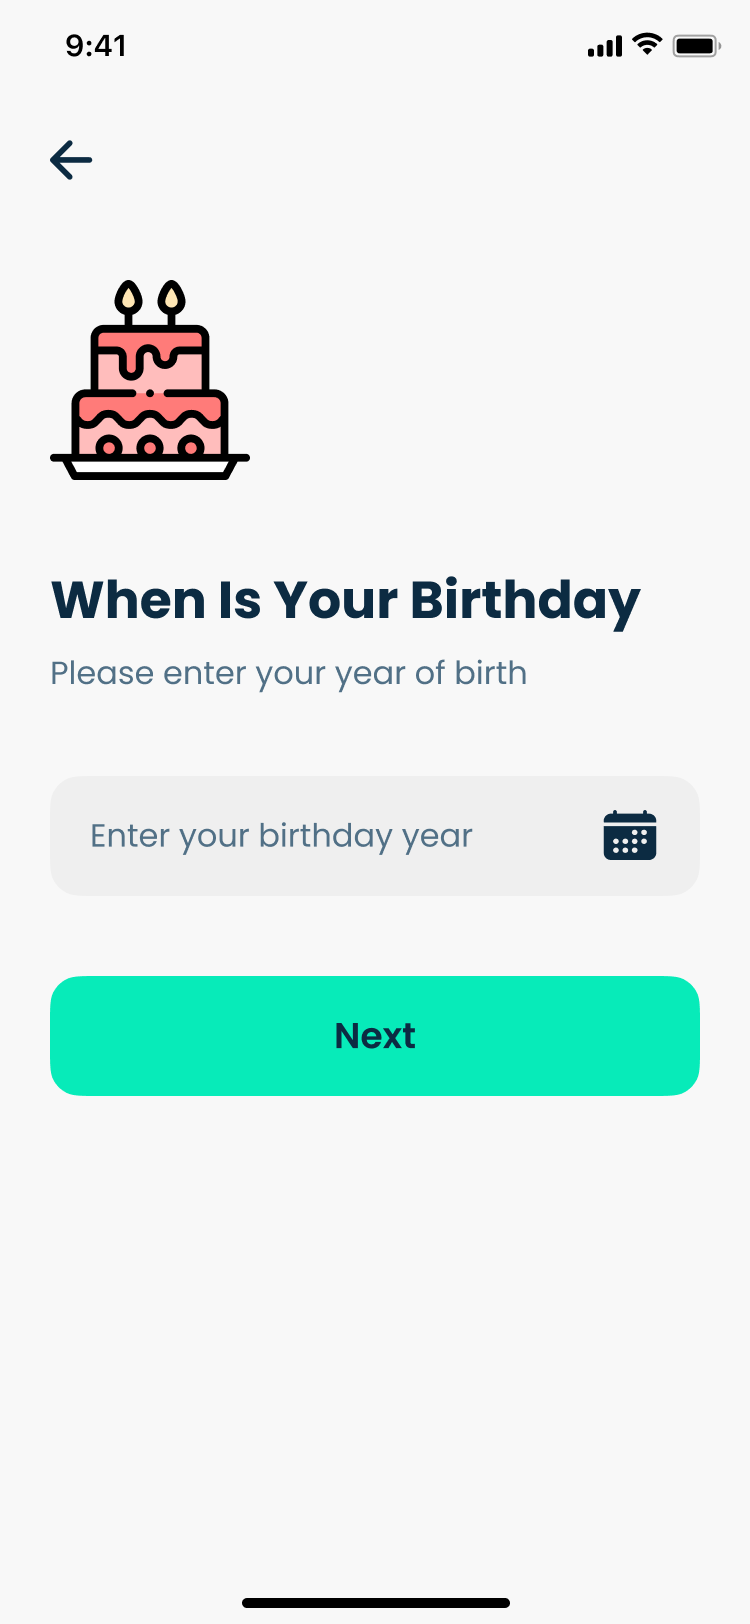
\includegraphics[height=10cm]{chapter_3/ui/New User Setup/002 - Birthday.png}
    \caption{หน้าการกรอกข้อมูลวันเกิด}
\end{figure}
\begin{figure}
    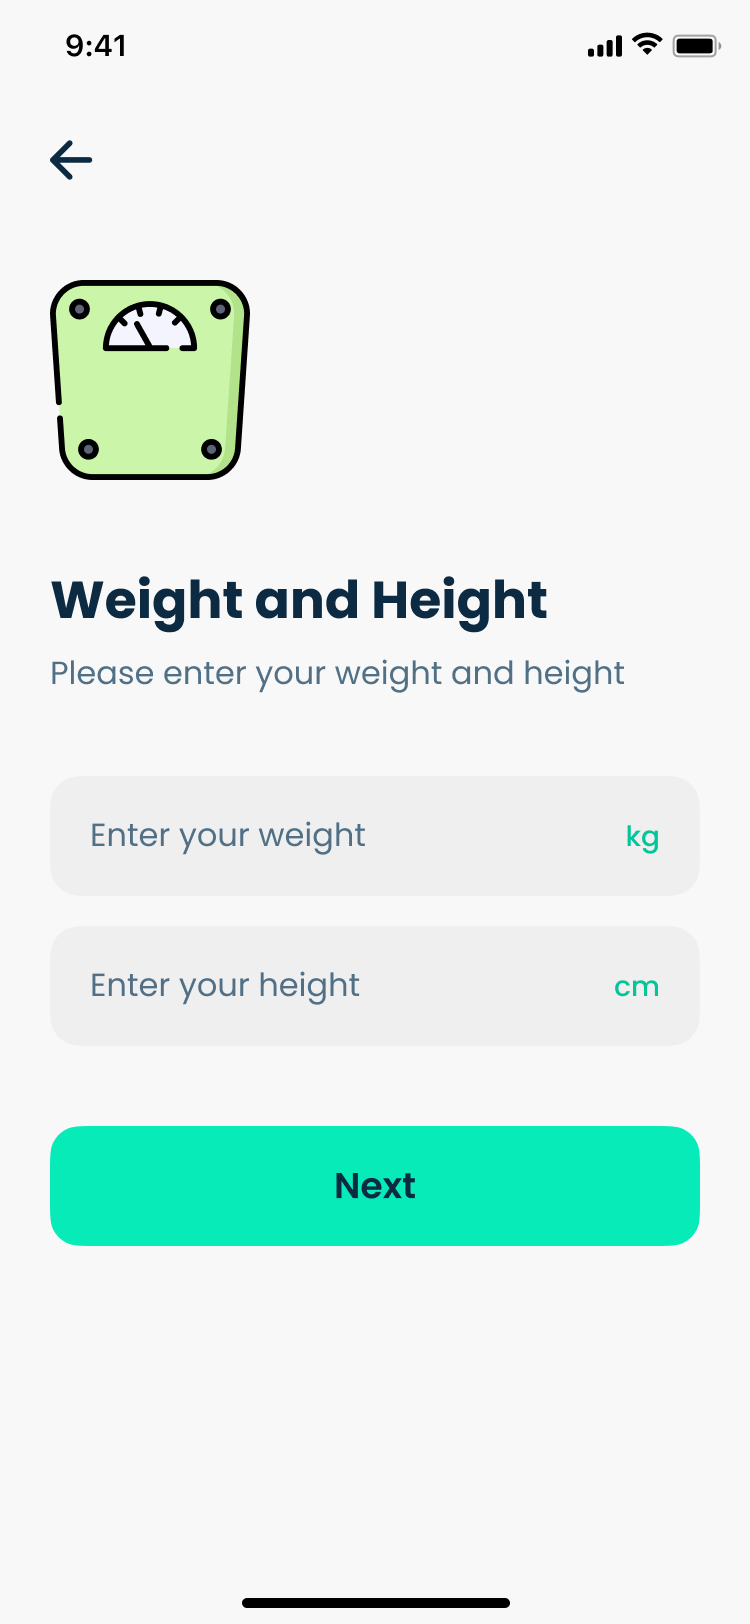
\includegraphics[height=10cm]{chapter_3/ui/New User Setup/003 - Weight and Height.png}
    \caption{หน้าการกรอกข้อมูลน้ำหนักและส่วนสูง}
\end{figure}
\begin{figure}
    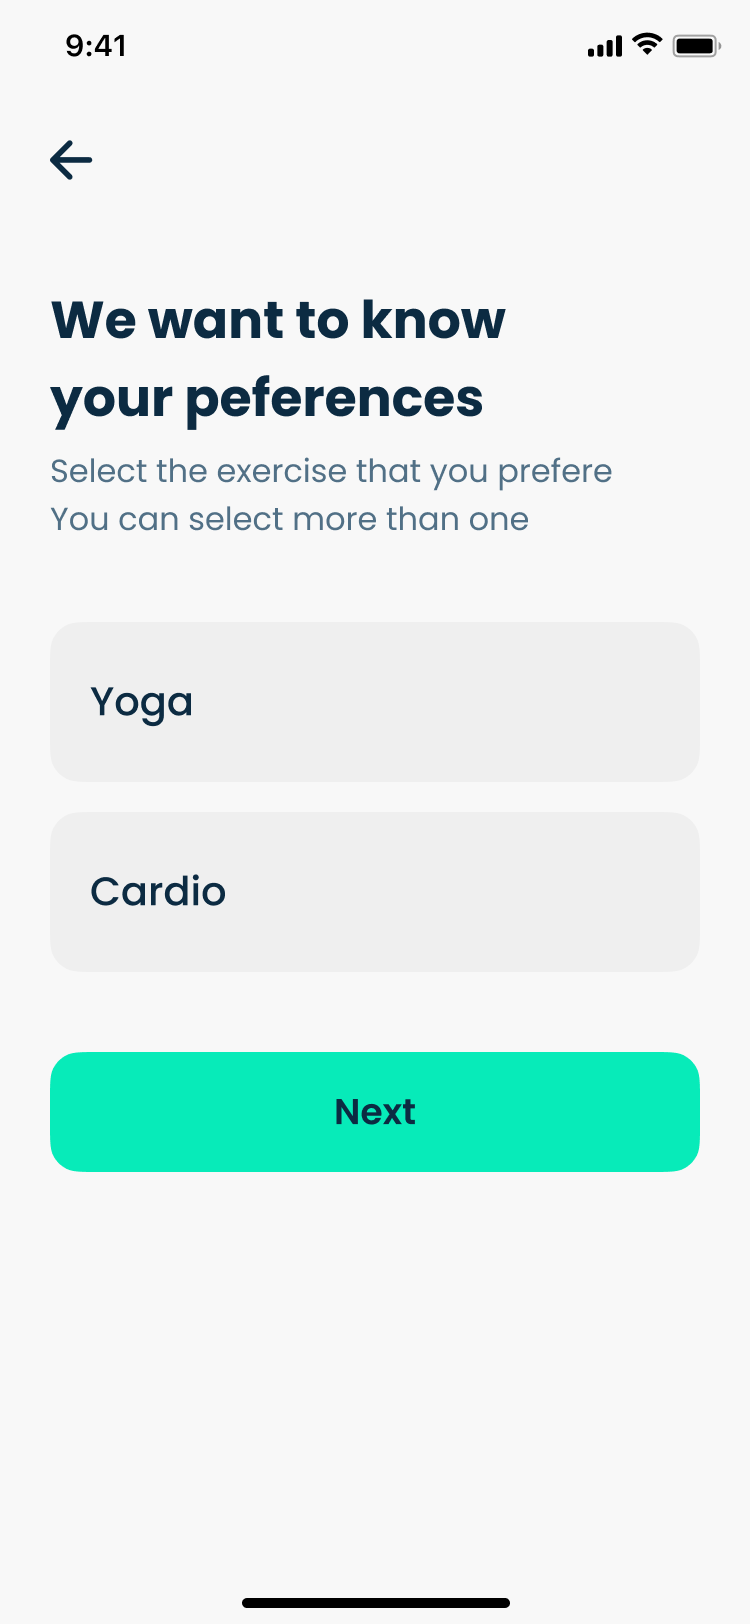
\includegraphics[height=10cm]{chapter_3/ui/New User Setup/004 - Exercise Preferences.png}
    \caption{หน้าการระบุประเภทของการออกกำลังกายที่ชื่นชอบ}
\end{figure}
\begin{figure}
    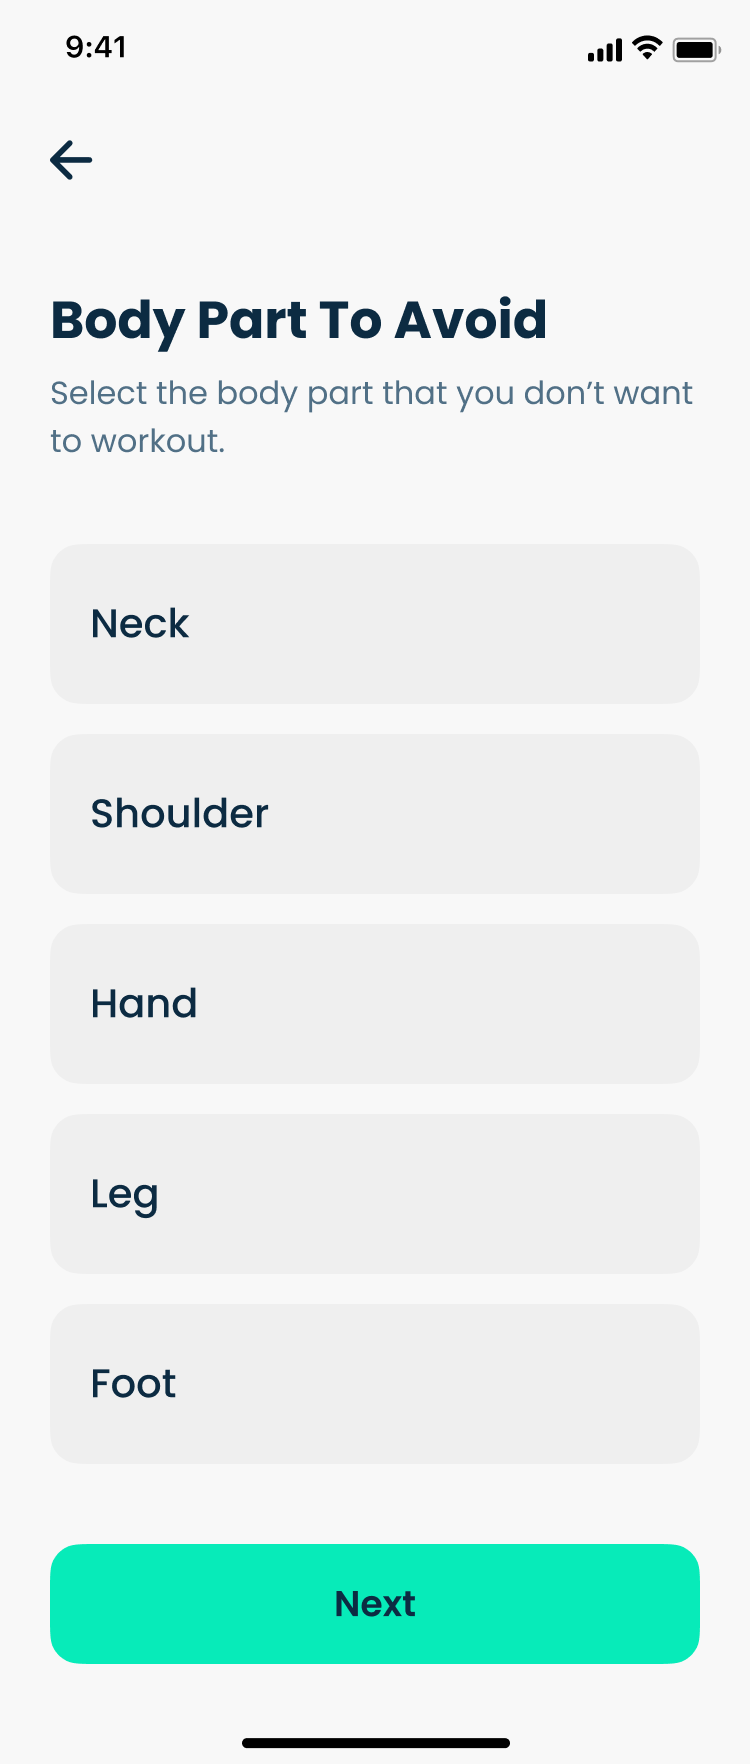
\includegraphics[height=10cm]{chapter_3/ui/New User Setup/005 - Exercise Preferences.png}
    \caption{หน้าการระบุส่วนของร่างกายที่ต้องการหลีกเลี่ยง}
\end{figure}
\begin{figure}
    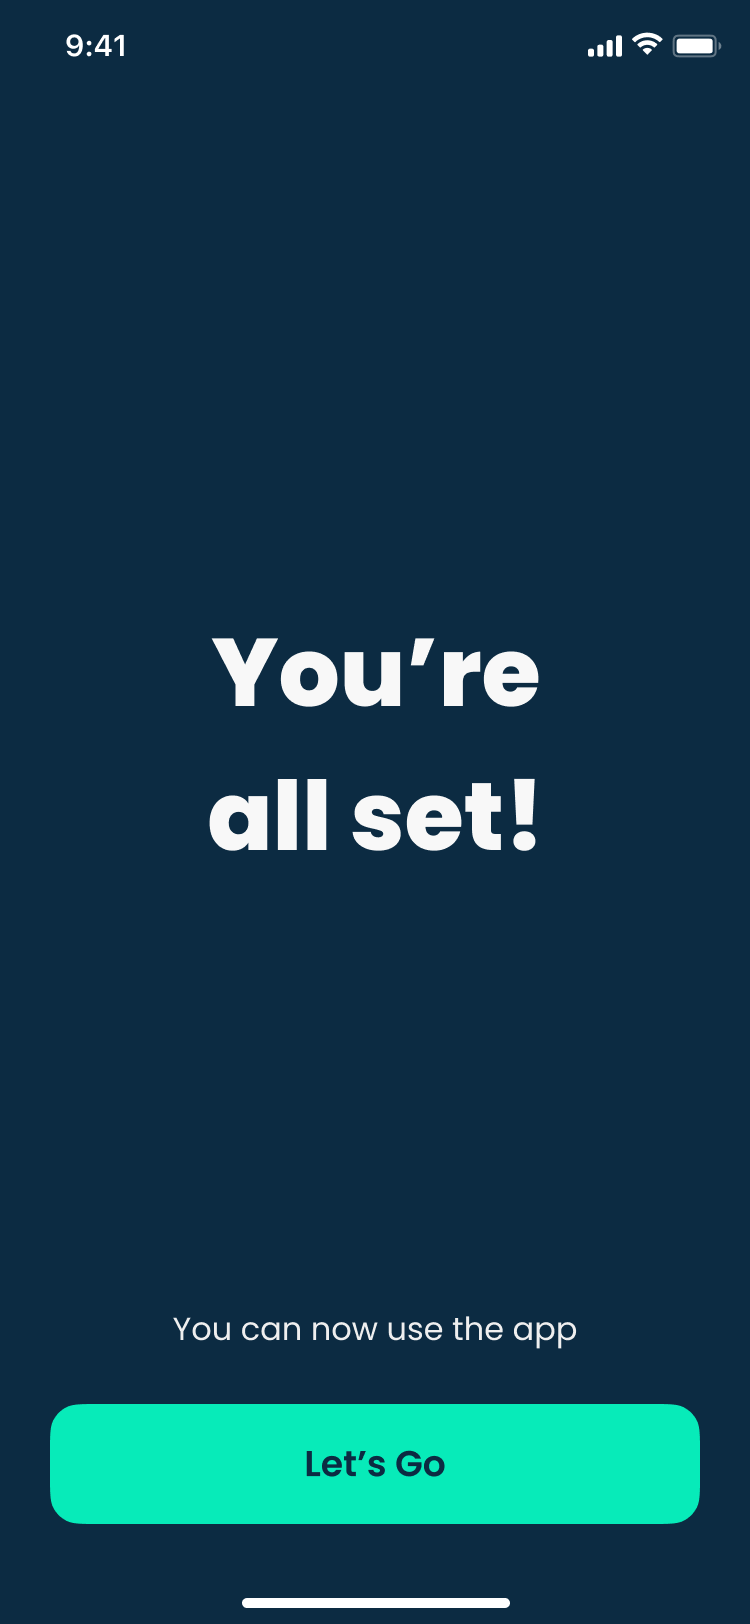
\includegraphics[height=10cm]{chapter_3/ui/New User Setup/006 - Complete.png}
    \caption{หน้าหลังจากการตอบคำถามความต้องการออกกำลังกาย}
\end{figure}

\subsection{หน้าแรกของแอปพลิเคชัน}
หน้าแรกของแอปพลิเคชัน จะแสดงผลคอร์สต่าง ๆ ที่เป็นที่นิยม และเหมาะสมสำหรับผู้ใช้ และแถบ Banner สำหรับการประชาสัมพันธ์คอร์สหรือข่าวสารต่าง ๆ ของทางแอปพลิเคชัน และด้านมุมบนขวาจะมีปุ่มค้นหา โดยจะสามารถค้นหาคอร์ส และบัญชีผู้ใช้ในระบบได้
\begin{figure}
    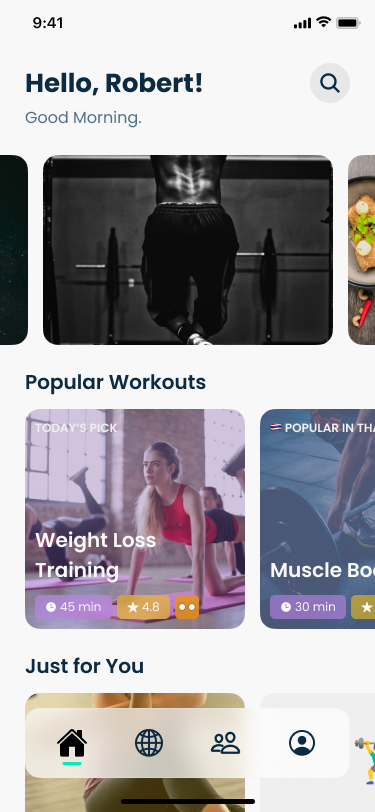
\includegraphics[height=10cm]{chapter_3/ui/Home.png}
    \caption{หน้าแรกของแอปพลิเคชัน}
\end{figure}

\subsection{หน้ากิจกรรมของผู้ใช้}
หน้ากิจกรรมของผู้ใช้ จะแสดงความเคลื่อนไหวต่าง ๆ ของบุคคลที่ผู้ใช้ได้ติดตามไว้ ผู้ใช้สามารถกด Reaction และ Comment กิจกรรมของบุคคลนั้น ๆ ได้ ด้านมุมขววาบนจะเป็นปุ่มตารางคะแนน Leaderboard ซึ่งจะสามารถให้ผู้ใช้ดูคะแนนสะสมของบัญชีที่ผู้ใช้ติดตามได้ และสามารถเปรียบเทียบคะแนนกับผู้ใช้ทั้งหมดในระบบได้
\begin{figure}
    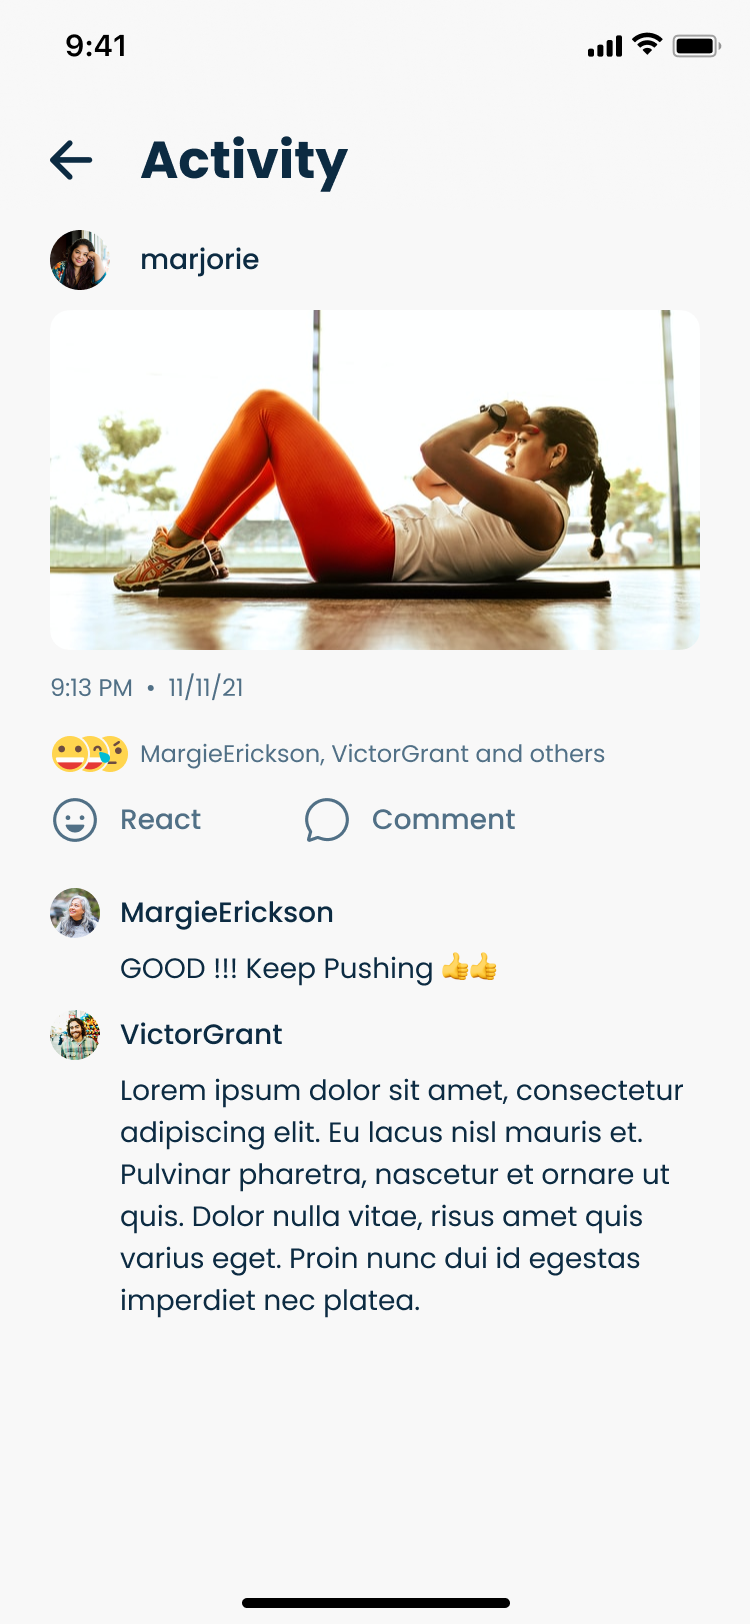
\includegraphics[height=10cm]{chapter_3/ui/Social/Activity.png}
    \caption{หน้ากิจกรรมของผู้ใช้}
\end{figure}
\begin{figure}
    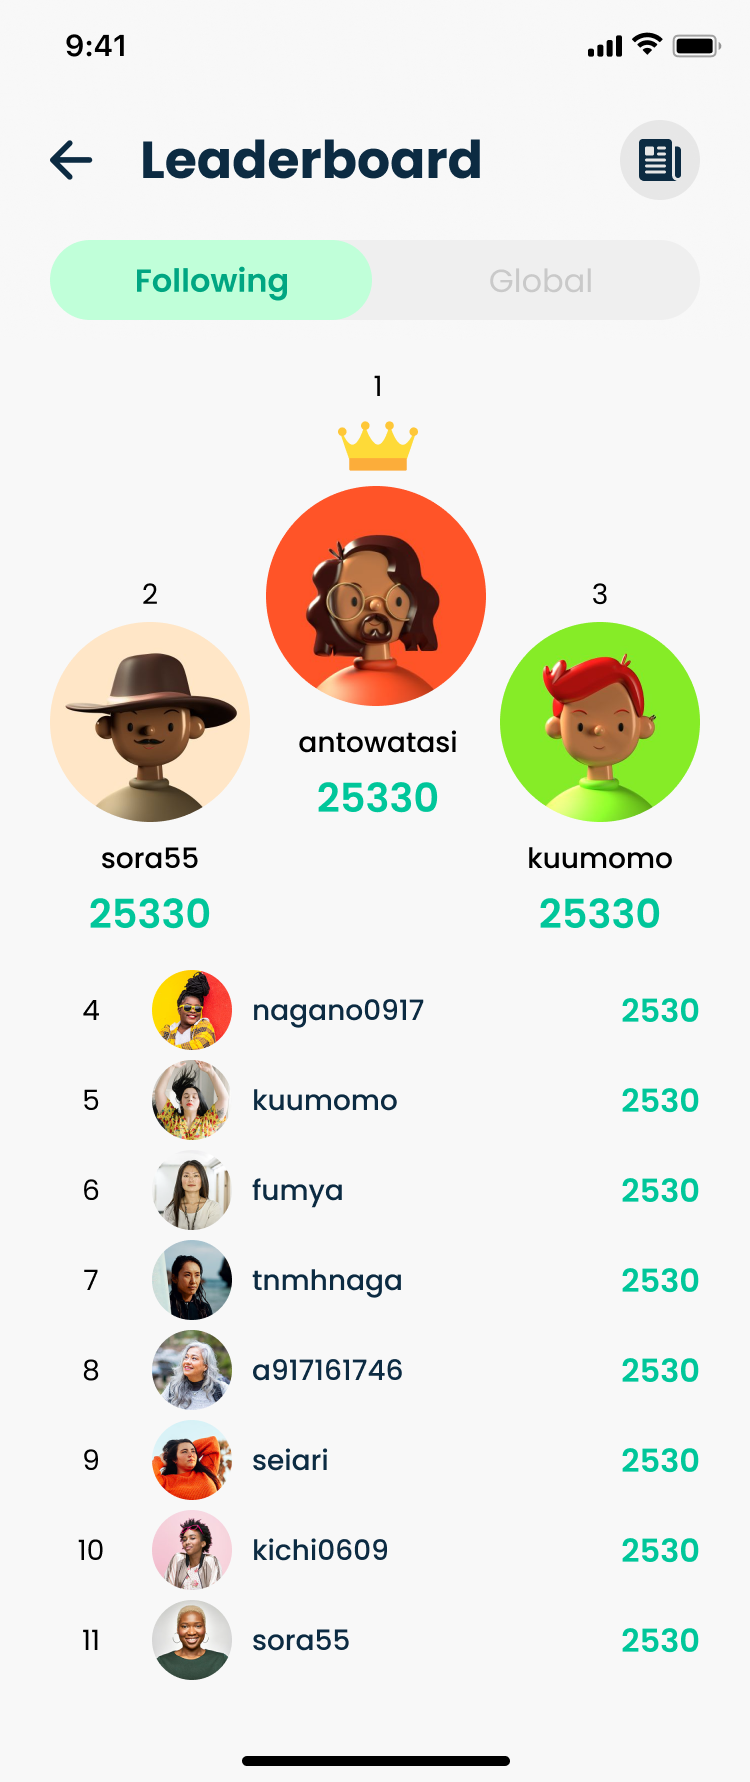
\includegraphics[height=10cm]{chapter_3/ui/Social/Leaderboard.png}
    \caption{หน้าตารางคะแนน Leaderboard}
\end{figure}

\subsection{หน้าข่าวสาร}
หน้าข่าวสารของแอปพลิเคชัน ซึ่งจะให้ผู้ใช้สามารถดูข่าวสารด้านการออกกำลังกายได้ และสามารถกดปุ่มชื่นชอบบทความได้
\begin{figure}
    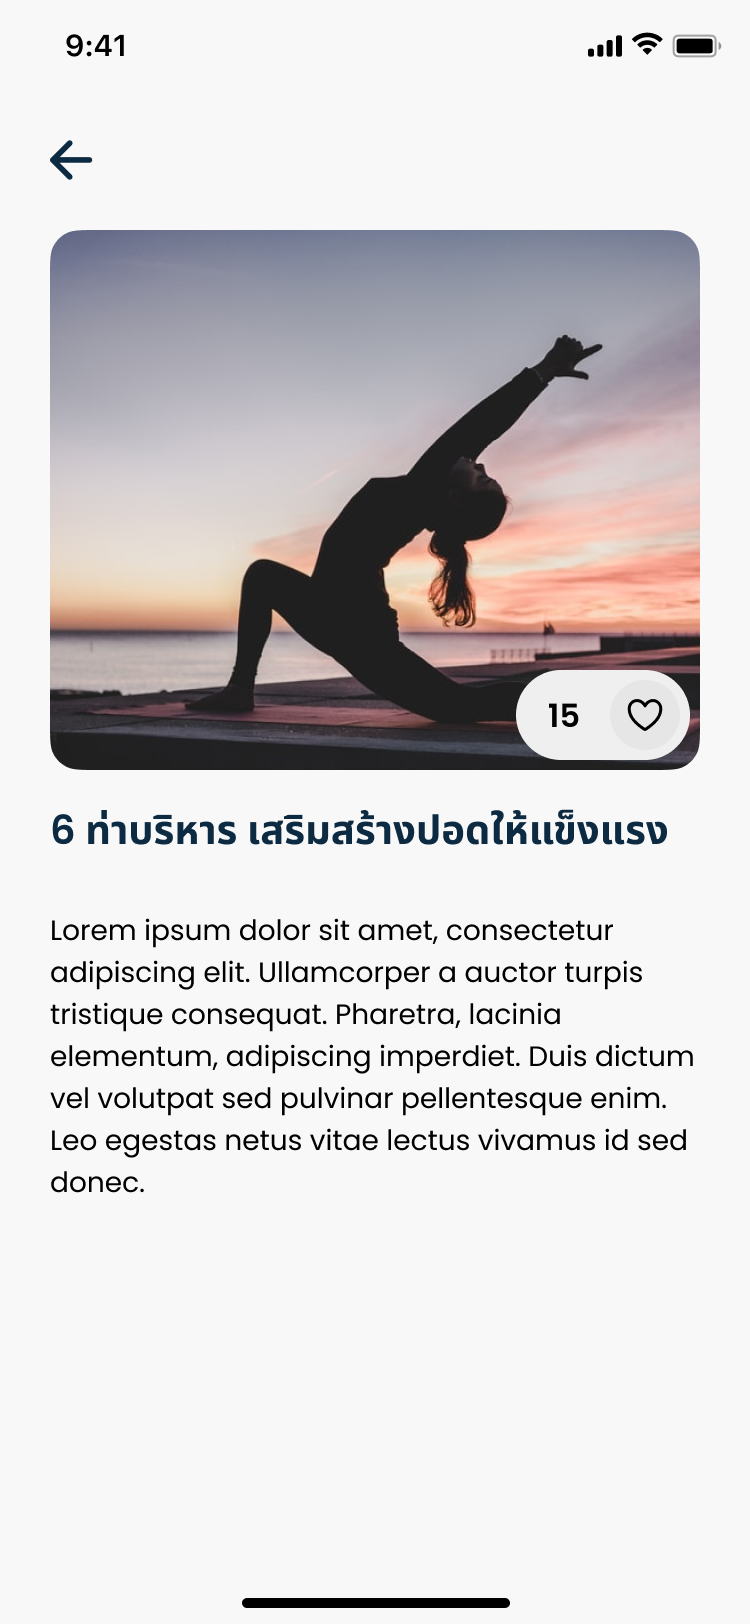
\includegraphics[height=10cm]{chapter_3/ui/News.png}
    \caption{หน้าข่าวสารของแอปพลิเคชัน}
\end{figure}

\subsection{หน้าการออกกำลังกาย}
หน้าการออกกำลังกาย ในหน้าแรกจะแสดงรายละเอียดคอร์ส รวมถึงคะแนนจากผู้ใช้ ระยะเวลาที่ใช้ และระดับความยากของคอร์ส เมื่อผู้ใช้กดปุ่มเริ่มการออกกำลังกาย ระบบจะแนะนำให้ผู้ใช้ทำท่าทางตามที่กำหนด โดยจะมีรายละเอียดแสดงอยู่ทางด้านบน และจะมีการแสดงข้อความแนะนำการปรับปรุงท่าทางการออกกำลังกายให้แก่ผู้ใช้
\begin{figure}
    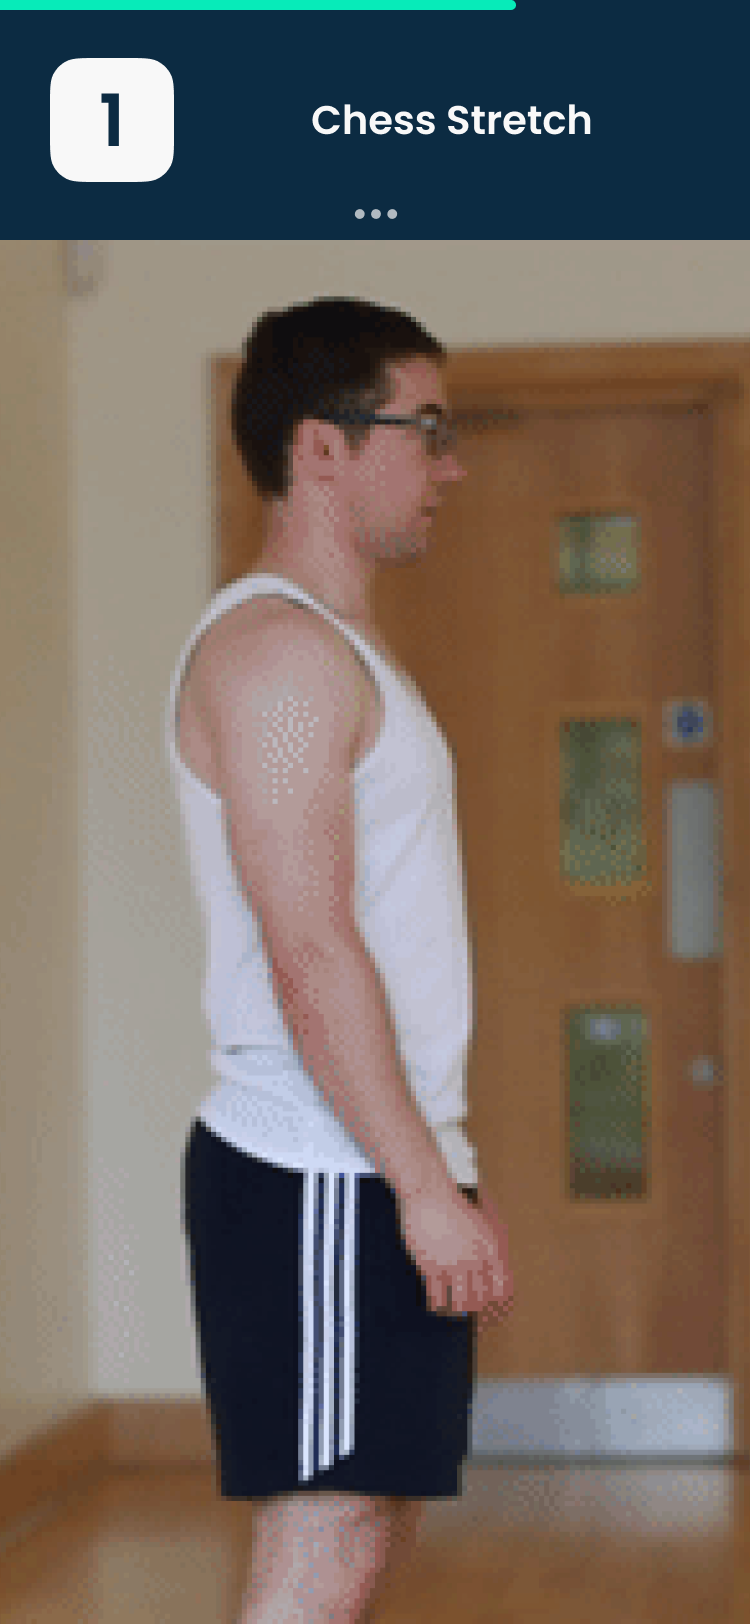
\includegraphics[height=10cm]{chapter_3/ui/Exercise/Step Begin.png}
    \caption{หน้าการสอนท่าทางให้แก่ผู้ใช้}
\end{figure}

\begin{figure}
    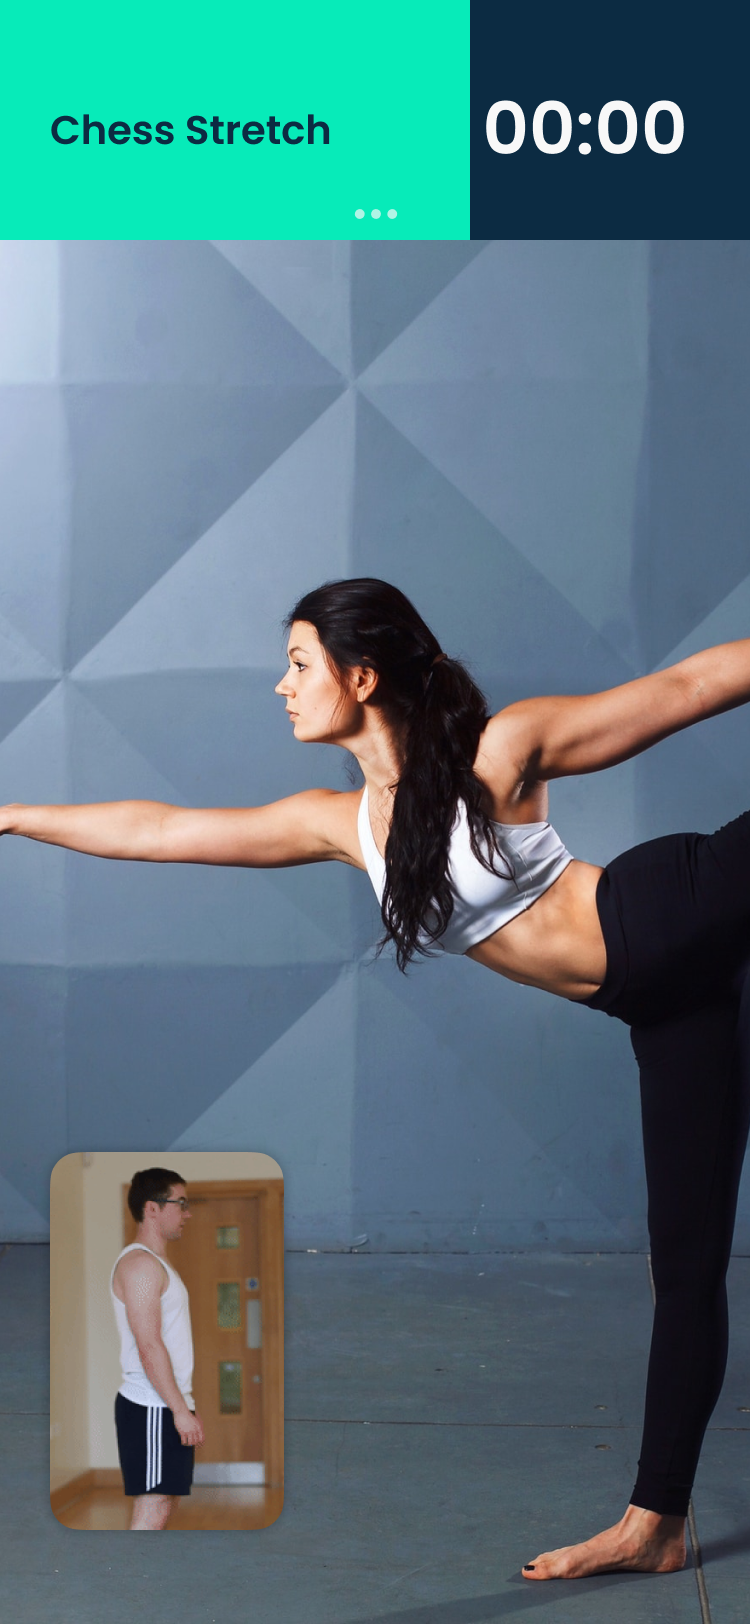
\includegraphics[height=10cm]{chapter_3/ui/Exercise/Step Counting.png}
    \caption{หน้าการออกกำลังกายที่จับเวลาให้ผู้ใช้ออกท่าทางค้างไว้ในเวลาที่กำหนด}
\end{figure}

\begin{figure}
    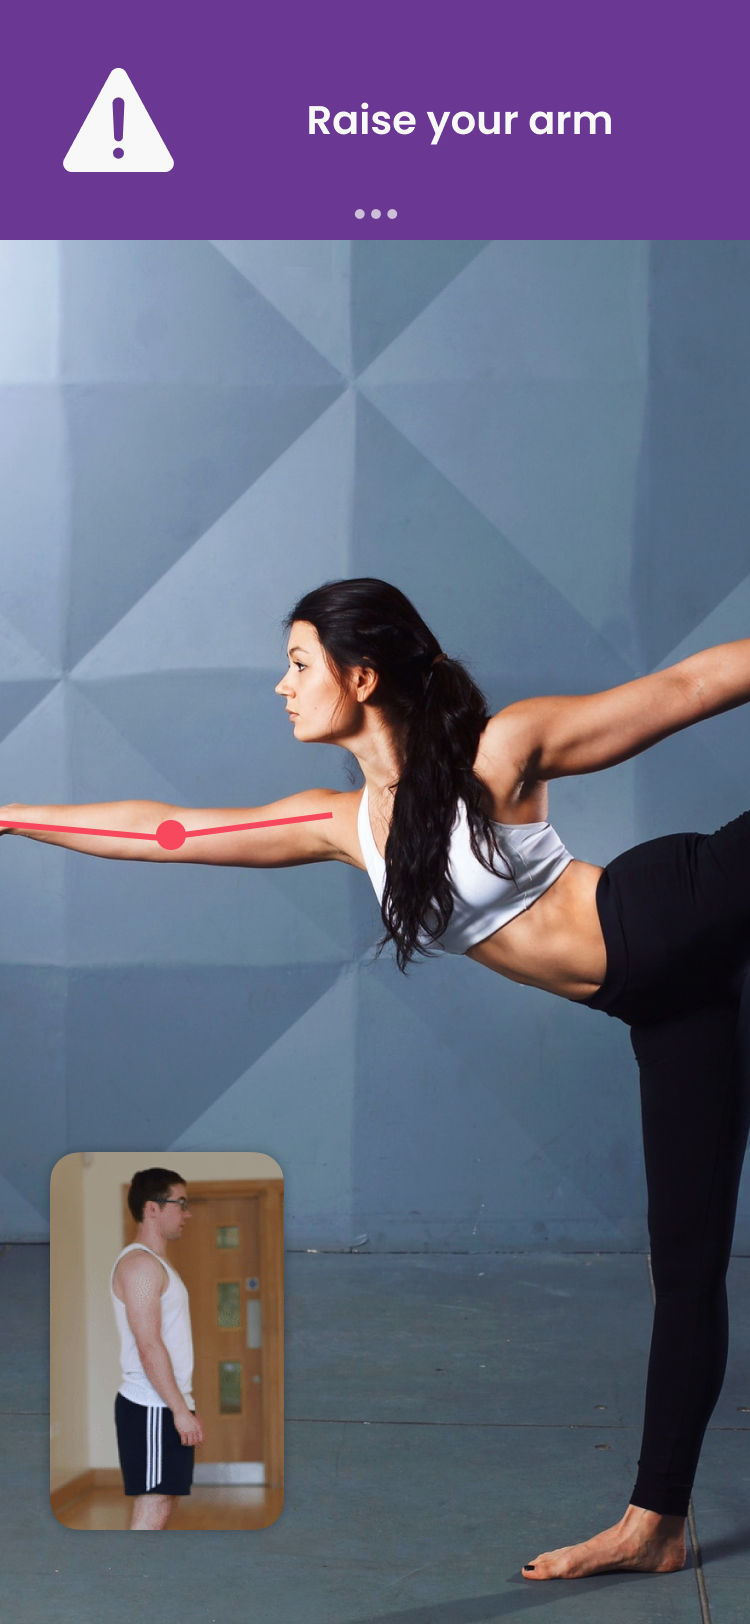
\includegraphics[height=10cm]{chapter_3/ui/Exercise/Warning.png}
    \caption{หน้าการแนะนำการปรับปรุงท่าทางให้แก่ผู้ใช้}
\end{figure}

\begin{figure}
    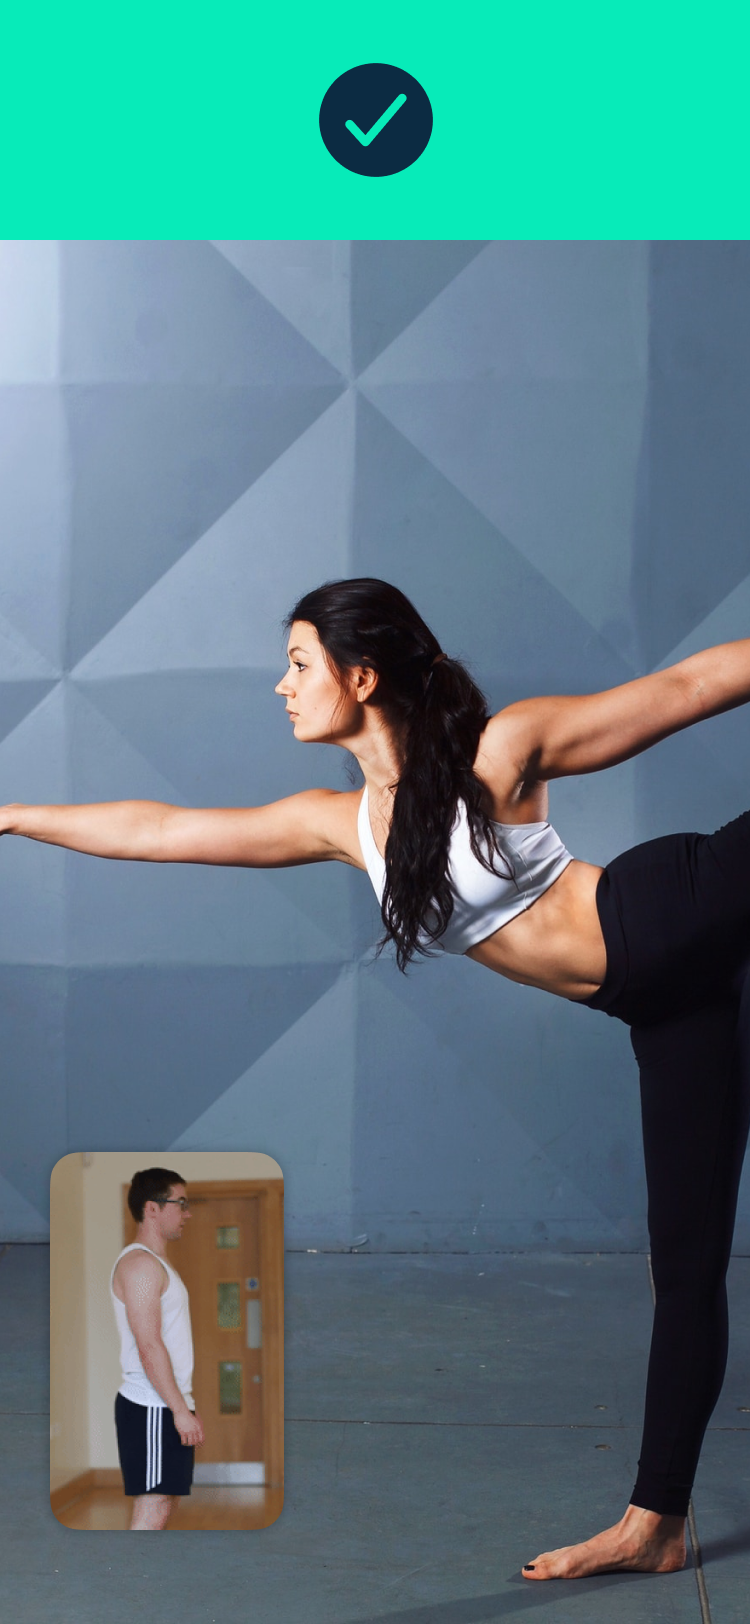
\includegraphics[height=10cm]{chapter_3/ui/Exercise/Step Finish.png}
    \caption{หน้าเมื่อเสร็จสิ้นการออกกำลังกาย}
\end{figure}

\subsection{หน้าบัญชีผู้ใช้}
หน้าบัญชีของผู้ใช้ ให้ผู้ใช้สามารถดูข้อมูลส่วนตัวของตนเองได้ รวมถึงดูเหรียญรางวัลเสมือนของตนเองได้

\begin{figure}
    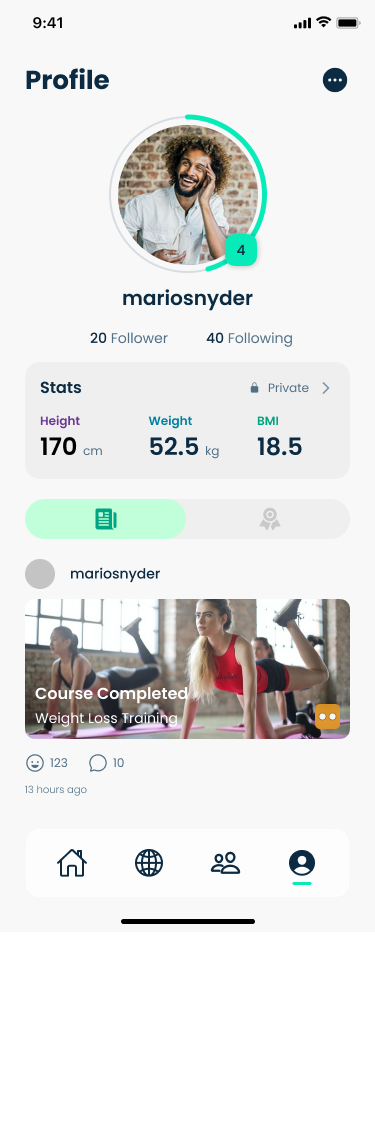
\includegraphics[height=10cm]{chapter_3/ui/Profile.png}
    \caption{หน้าบัญชีของผู้ใช้}
\end{figure}


\clearpage